\section{Proposed Research and Timeline}
To start the research for my PhD thesis I seek to explore phonon softening and charge ordering phenomena in \ts.
Former work of the Siwick Group on \ts\space shows that photoexciting carriers into the 3d conduction band leads to a stiffening of transverse phonons at the M points\cite{otto2021}.
The coupling between free carriers and phonons, however, is not enhanced.
This is in striking contrast to the behavior observed in graphite\cite{stern2018}.
Both experiment were conducted at room temperature.
The \ac{CDW} phase with its excitonic ground state should be fragile against large densities of free charge carries due to screening effects.
It would be interesting to investigate the dynamics of the excitonic ground state decaying upon photo-excitation and its subsequent reformation upon cooling, while systematically varying the pump-fluence.
At this point in time it is not possible to control the temperature of the sample.

The installation of a closed-cycle cryostat is currently ongoing at will allow access to sample temperatures of 4-XXX\,K.
In addition to that, the machine is subject to more upgrades.
First, we have reduced the physical length of the instrument, reducing the influence of space-charge effects of the electron bunch on the time resolution.
Second, a Faraday cup has been designed and machined and is ready for installation to measure number of electrons in the bunches.
This allows for further characterization and better control of the instrument.
Third, a new detector camera (Dectris Quadro) has been installed and implemented in the laboratory software system.
Instead of a conventional CCD chip coupled to a scintillator, the detector is a \emph{hybrid pixel detector} consisting of bare silicon pixels that can directly count incoming electrons.
Signal-to-noise ratio \textbf{radically} improved and the read-out electronics are fast enough to capture diffraction images of every single electron bunch.
In addition to that the high dynamic range makes the use of a beam stop obsolete; the full diffraction pattern can be captured an analyzed.
Finally, the Dectris Quadro is much less sensitive to scattered light from pump and probe beam, which helps to produce diffraction images with less distortions.

The previous work performed on \ts\space in the Siwick Group combined with ne new capabilities of the modified experimental setup provide a solid base to investigate the \ac{CDW} phase transition in new ways.
At a later stage it could be promising to not only probe the $\Gamma\mathrm{MK}$ plane of the \ac{BZ}, but also access the L point.
The problem of forfeiting time resolution has been overcome by other groups encountering similar issues in time-resolved diffraction experiments.
The idea is to compensate the velocity mismatch of pump and probe pulse by tilting the optical pump pulse.
This leads to synchronous time delay of pump and probe event across the whole sample area\cite{baum2006,zhou2013}.
While conducting experiments on tilted samples without introducing a tilt to wave front of the pump pulse, it would enhance the data quality considerably.

\begin{figure}[!t]
	\begin{minipage}{0.5\columnwidth}
		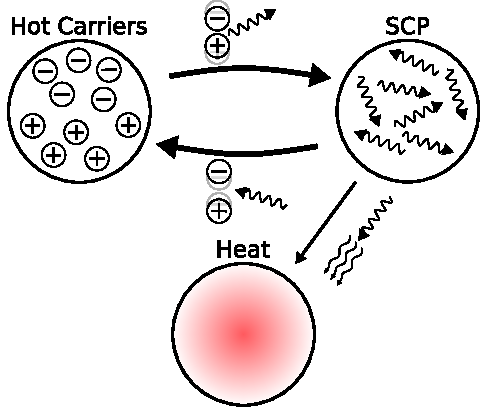
\includegraphics[width=\columnwidth]{figs/phonon_bottleneck.pdf}
	\end{minipage}
	\hspace{0.04\columnwidth}
	\begin{minipage}{0.45\columnwidth}
		\caption{Schematic of the phonon bottleneck model with three interactions and three reservoirs, namely hot carriers, strong coupling phonons (SCPs) and heat. Free carriers can form and exciton while emmiting a SCP. Vice versa phonons can be absorbed by an exciton, creating a pair of hot carriers. The last transition describes anharmonic decay of SCPs into different phonon populations that are regarded to as heat.}
		\label{fig:model}
	\end{minipage}
\end{figure}

\subsection*{Timeline}
My goal is to submit my PhD thesis at the end of 2025, which would correspond to an overall duration of four years.
The first half of this year will be primarily devoted to machine upgrades, data collection and simulations on the low-temperature phase of \ts.
With the temperature controllable sample stage being ready in summer, the third quarter of the 2022 can be spent on collecting a comprehensive dataset of the decay and formation dynamics of the low temperature phase of \ts.
In the mean-time I am working on the calculation on the one-phonon structure factor of the low temperature phase.
The 2$\times$2$\times$2 lattice recontruction leads to an 8-fold increase in atoms per unit cell, which is making these simulations particularly challening.
Data analysis and preparation of a manustript should follow in the beginning of 2023.
After the first run of experiments I plan to further extend the machine capabilities and access the L points of the \ac{BZ}.
An \emph{Attocube} positions system is already available; the setup of a pulse-front tilting optical stage will require rather simple optical equipment, namely a grating, some mirrors, lenses and positioning tools.
With these extensions a new degree of freedom can be probed.
Depending on the results of the first experiment run, I might want to dig deeper into the mechanisms studied in the first run, or even look into related material systems.
A particularly interesting feature of \ts\space is, that upon intercalation with copper it will become superconducting below a critical temperature of 4.15\,K\cite{morosan2006}.

% hopefully present preliminary results in presentation
